% This file was created with matplot2tikz v0.5.4.
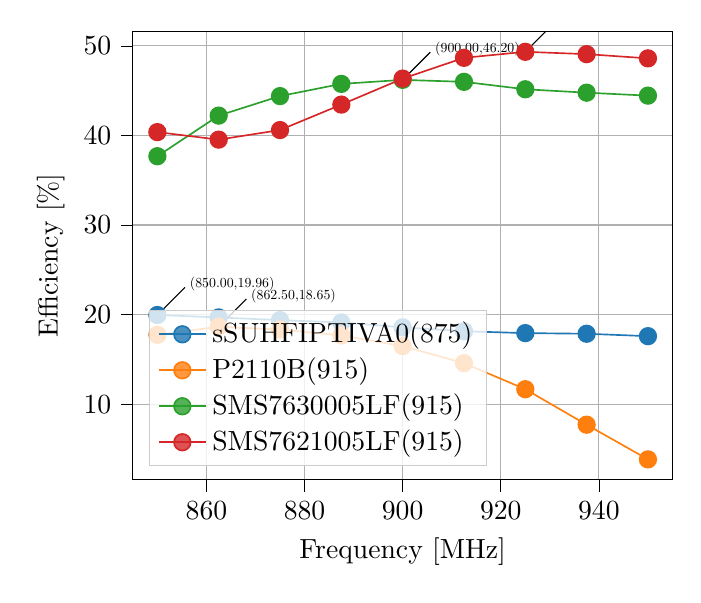
\begin{tikzpicture}

\definecolor{crimson2143940}{RGB}{214,39,40}
\definecolor{darkgray176}{RGB}{176,176,176}
\definecolor{darkorange25512714}{RGB}{255,127,14}
\definecolor{forestgreen4416044}{RGB}{44,160,44}
\definecolor{lightgray204}{RGB}{204,204,204}
\definecolor{steelblue31119180}{RGB}{31,119,180}

\begin{axis}[
legend cell align={left},
legend style={
  fill opacity=0.8,
  draw opacity=1,
  text opacity=1,
  at={(0.03,0.03)},
  anchor=south west,
  draw=lightgray204
},
tick align=outside,
tick pos=left,
x grid style={darkgray176},
xlabel={Frequency [MHz]},
xmajorgrids,
xmin=845, xmax=955,
xtick style={color=black},
y grid style={darkgray176},
ylabel={Efficiency [\%]},
ymajorgrids,
ymin=1.576, ymax=51.604,
ytick style={color=black}
]
\addplot [semithick, steelblue31119180, mark=*, mark size=3, mark options={solid}]
table {%
850 19.96
862.5 19.69
875 19.39
887.5 19.13
900 18.59
912.5 18.15
925 17.94
937.5 17.87
950 17.6
};
\addlegendentry{sSUHFIPTIVA0(875)}
\addplot [semithick, darkorange25512714, mark=*, mark size=3, mark options={solid}]
table {%
850 17.75
862.5 18.65
875 18.34
887.5 17.68
900 16.49
912.5 14.59
925 11.68
937.5 7.72
950 3.85
};
\addlegendentry{P2110B(915)}
\addplot [semithick, forestgreen4416044, mark=*, mark size=3, mark options={solid}]
table {%
850 37.68
862.5 42.21
875 44.39
887.5 45.75
900 46.2
912.5 45.98
925 45.15
937.5 44.77
950 44.44
};
\addlegendentry{SMS7630005LF(915)}
\addplot [semithick, crimson2143940, mark=*, mark size=3, mark options={solid}]
table {%
850 40.37
862.5 39.53
875 40.6
887.5 43.44
900 46.34
912.5 48.66
925 49.33
937.5 49.07
950 48.6
};
\addlegendentry{SMS7621005LF(915)}
\draw[->,draw=black] (axis cs:850,19.96) ++(10pt,10pt) -- (axis cs:850,19.96);
\draw (axis cs:850,19.96) ++(10pt,10pt) node[
  scale=0.5,
  anchor=base west,
  text=black,
  rotate=0.0
]{(850.00,19.96)};
\draw[->,draw=black] (axis cs:862.5,18.65) ++(10pt,10pt) -- (axis cs:862.5,18.65);
\draw (axis cs:862.5,18.65) ++(10pt,10pt) node[
  scale=0.5,
  anchor=base west,
  text=black,
  rotate=0.0
]{(862.50,18.65)};
\draw[->,draw=black] (axis cs:900,46.2) ++(10pt,10pt) -- (axis cs:900,46.2);
\draw (axis cs:900,46.2) ++(10pt,10pt) node[
  scale=0.5,
  anchor=base west,
  text=black,
  rotate=0.0
]{(900.00,46.20)};
\draw[->,draw=black] (axis cs:925,49.33) ++(10pt,10pt) -- (axis cs:925,49.33);
\draw (axis cs:925,49.33) ++(10pt,10pt) node[
  scale=0.5,
  anchor=base west,
  text=black,
  rotate=0.0
]{(925.00,49.33)};
\end{axis}

\end{tikzpicture}
